\chapter{2D Image Processing using the Graph Laplacian Operator}

\section{Theoretical basis}

\paragraph{}
Multiple image processing filters can be built by graph Laplacians. As Milanfar mentions in \cite{siam_slides_2016}, smoothing, deblurring, sharpening, dehazing, and other filters can be created.
Laplacians can also be used for compression artifact removal, low-light imaging and image segmentation.

As it is known, an image filter consists of a function which outputs one pixel, taking all pixels as input and applying weights to them. We can write this as
\[z_i = \sum_j W_{ij}y_j,\]
\(z_i\) being the output pixel, \(W_{ij}\) the weight and \(y_j\) all input pixels.
This means that we have a vector of weights for each pixel.

So, as a practical notation, we can say that, with \(W\) the matrix of weights and \(y\) the input image as a vector,
\[z = Wy.\]

\paragraph{}
Now we want to represent the image as a graph.
Each pixel is a node and has edges to multiple other nodes.
We can arbitrarily define how the pixels connect to each other, so we can say that the graph is complete, each node connects to all other nodes.
We can weigh the edges to measure the similarity between pixels.

\paragraph{}
Affinity, or similarity, is a subjective term which we can also define as we need.
Pixels can be similar if they are spatially close or if they have the same color, or both.
These similarities give us the so-called affinity matrix \(K\).

\paragraph{}
By extending this affinity matrix, we obtain the graph Laplacian \(\Lapl\).
And we use the latter to build the filter \(W\) containing the weights.

\paragraph{}
According to \cite{modern_tour_2013}, to build a denoising filter from the Laplacian, we have
\[\Lapl = I - W.\]
The graph Laplacian has multiple definitions, but the simplest is the unnormalised one:
\[\Lapl_U = D - K,\]
with \(D\) a positive definite diagonal matrix with the normalising factors along its diagonal such as \(\forall i, D = diag\{\sum_j K_{ij}\}\).
\(D\) corresponds in fact to the degrees of each node in graph theory terminology.
Other definitions of the Laplacian are shown later in~\ref{subsec:laplacian-variations}.

\paragraph{}
Interestingly, we can define from \cite{glide_2014} that, by approximating \(W\) by a symmetric, positive definite, doubly-stochastic matrix, this new \(\hat{W}\) can be computed thanks to its eigendecomposition

\[\hat{W} = VSV^T,\]
\(V\) being the eigenvectors and \(S\) the eigenvalues as a diagonal matrix.

Our global filter can be expressed as
\[\hat{z} = \hat{W}y = VSV^Ty.\]

This will be useful since the filter matrix \(W\) becomes huge very quickly and we will need a way to approximate it. Indeed, \(W\) is a square matrix with \(n*n\) elements, \(n\) the number of pixels in the picture.

\paragraph{Approximation by Nystr\"om Extension}

To compute the filter, the first matrix that is needed is the affinity matrix \(K\).
Both matrices have the same size and are computationally expensive.

That is why we approximate the affinity matrix by sampling the picture.
We sample \(p\) pixels, such as  \(p << n\). Different sampling techniques exist and are shown in~\ref{subsec:sampling-variations}.

Once sampled, we compute \(K_A\) and \(K_B\), which are parts of \(K\) such as
\[
 K = \begin{bmatrix}
  K_A & K_B \\
  K_B^T & K_C
 \end{bmatrix}.
\]
\(K_A\) represents the affinity matrix of size \(p*p\) between the sample pixels, whereas \(K_B\) is the affinity matrix of size \(p*m\), such as \(m = n-p\), between the sample pixels and the remaining pixels.

These matrices will be computed thanks to a kernel function (or affinity function). This can be the bilateral filter, non-local means or another, as shown in~\ref{subsec:kernel-variations}.

Once computed, we can approximate the eigenvectors \(\Phi\) and eigenvalues \(\Pi\) of \(K\) thanks to the eigendecomposition of \(K_A\).

As stated in \cite{glide_2014}, we can define the decomposition of \(K_A\)
\[K_A = \Phi_A \Pi_A \Phi_A^T\]
and the approximation of \(K\) such as
\[\tilde{K} = \tilde{\Phi} \Pi_A \tilde{\Phi}^T\]
and finally the approximation of the \(p\) first eigenvectors of \(K\)
\[
 \tilde{\Phi} = \begin{bmatrix}
  \Phi_A \\
  K_B^T \Phi_A \Pi_A^{-1}
 \end{bmatrix}
\]

One might wonder how an approximation of the first elements of the eigendecomposition can be enough to approximate the whole matrix.
In fact, the eigenvalues decay quickly as shown in \cite{siam_slides_2016} and \cite{meyer_perturbation_2014}. This means that the whole matrix is mainly defined by the first eigenelements.

\paragraph{Orthogonalisation}
From this eigendecomposition approximation of \(K\), we can then approximate the eigenvectors and eigenvalues of \(W\).
Indeed, with the same procedure as for \(K\), we can first compute similarly \(W_A\) and \(W_B\) such as
\[
 W = \begin{bmatrix}
  W_A & W_B \\
  W_B^T & W_C
 \end{bmatrix}
\]

We could apply the Nystr\"om extension again, but the resulting eigenvectors are not orthonormal.
To approximate orthonormal eigenvectors, we can use the proposed method by \cite{fowlkes_spectral_2004} which consists, if \(W_A\) is positive definite, in computing a matrix \(Q\) such as
\[Q = W_A + W_A^{-\frac{1}{2}} W_B W_B^T W_A^{-\frac{1}{2}},\]
where \(W_A^{-\frac{1}{2}}\) is the inverse of the symmetric positive definite square root of \(W_A\).
By diagonalising \(Q\) we obtain \(Q = \Phi_Q \Pi_Q \Phi_Q^T\).
As it is proven in the appendix of \cite{fowlkes_spectral_2004}, \(\hat{W} = V\Pi_QV^T\) with
\[
 V = \begin{bmatrix}
  W_A \\
  W_B^T
 \end{bmatrix}
 W_A^{-\frac{1}{2}} \Phi_Q \Pi_Q^{-\frac{1}{2}}.
\]

\(V\) is a base of orthonormal eigenvectors where \(\forall i, V_i\) is the \(i\)-th eigenvector of \(\hat{W}\), which can numerically be shown by \(V^T V = I\), \(||V_i|| = 1\) and \(\forall j, i \neq j, V_i V_j = 0\).

\paragraph{Summary}

The figure below summarises the described processing chain.

\begin{figure}[H]
    \centering
    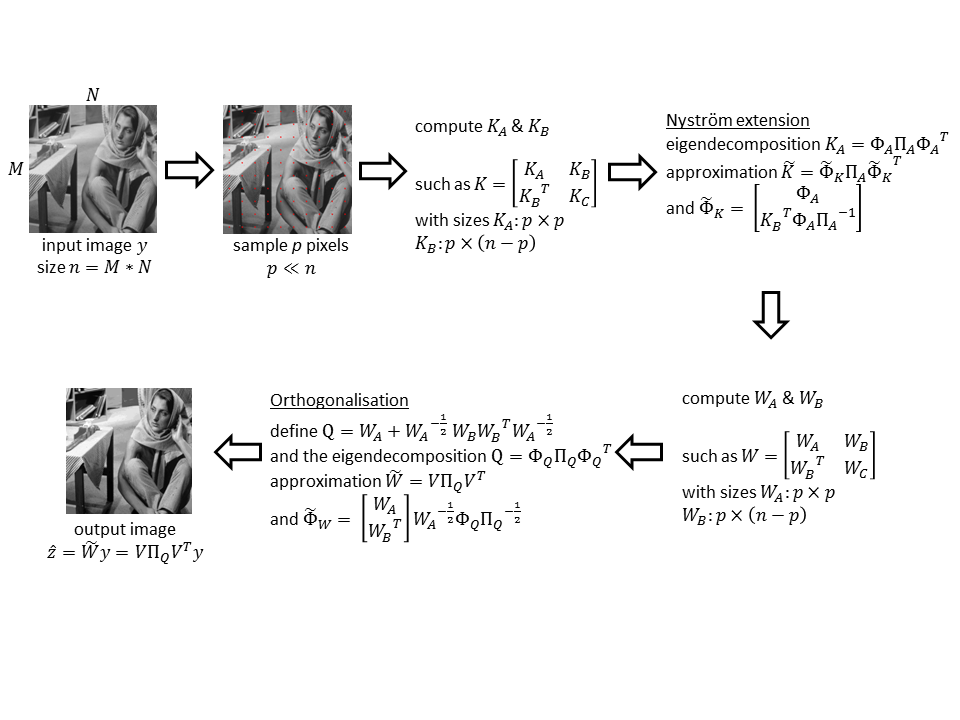
\includegraphics[width=1.2\textwidth]{img/processingChain.png}
    \caption{The 2D image processing chain}
\end{figure}

\section{First implementation}

\paragraph{Details}
The first implementation of this flow is aimed to denoise the input image.
This represent an early stage of the internship.
The sample pixels are selected in a spatially uniform manner.
It uses the NLM from \cite{buades_review_2005} as kernel method to compute the pixels similarity.
The Laplacian matrix is defined through the ``Sinkhorn" iterative algorithm \cite{milanfar_symmetrizing_2013}, where the resulting approximated eigenvectors require to be orthogonalised, which can be done in one step, as discussed in \cite{fowlkes_spectral_2004}.
We finally apply our approximated filter to the noisy image.

The implementation is generally inspired by the MatLab implementation of \cite{glide_2014}.

\paragraph{Results}
The results of this very first experiment are not yet totally satisfying as we can observe visually:

\begin{figure}[H]
    \centering
    \begin{subfigure}[b]{0.32\textwidth}
        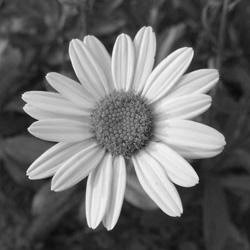
\includegraphics[width=\textwidth]{img/flowerOriginal.png}
        \caption{Original image}
    \end{subfigure}
    \begin{subfigure}[b]{0.32\textwidth}
        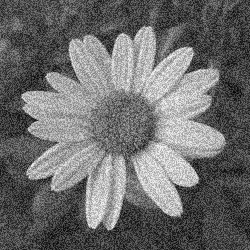
\includegraphics[width=\textwidth]{img/flowerNoisy.png}
        \caption{Noisy image (\(\sigma=100\))}
    \end{subfigure}
    \begin{subfigure}[b]{0.32\textwidth}
        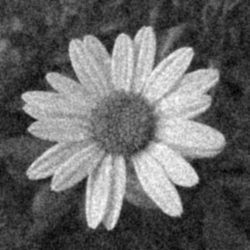
\includegraphics[width=\textwidth]{img/flowerOutput.png}
        \caption{Output image}
    \end{subfigure}
\end{figure}

We observe that the output picture is still quite noisy and blurry, we can certainly do better.
But still, as a first result, this is better than nothing.
The noise as been added artificially using a normal distribution of \(\sigma = 100\).

\section{Algorithm variations}

\subsection{Sampling method}
\label{subsec:sampling-variations}
The sample requires to represent only less than 1\% of the pixels of the image. To achieve this, we can use different approaches. The chosen method is decisive for the application of the Nystr\"om method.
\begin{description}[align=left]
 \item [Random sampling (RS)] most common and simple sampling scheme, but no deterministic guarantee of the output quality. Can produce good results for images with poor resolution, but with a huge amount of data, random sampling is limited because it cannot reflect the structure of the data set \cite{zhan_improved_2017}.
 \item [K-means sampling (KS)] associate to each pixel a 5-D space (R, G, B, X, Y) and divide the pixels into K clusters (K centers). These clusters are a good sampling scheme for images with simple and uniform backgrounds \cite{kao_sampling_2012} \cite{zhang_improved_2008}.
 \item [Uniform spatially sampling] the uniformity of the sample gives good results for image sampling because of the spatial correlation of pixels. This method remains simple but effective \cite{glide_2014}.
  \begin{figure}[H]
      \centering
      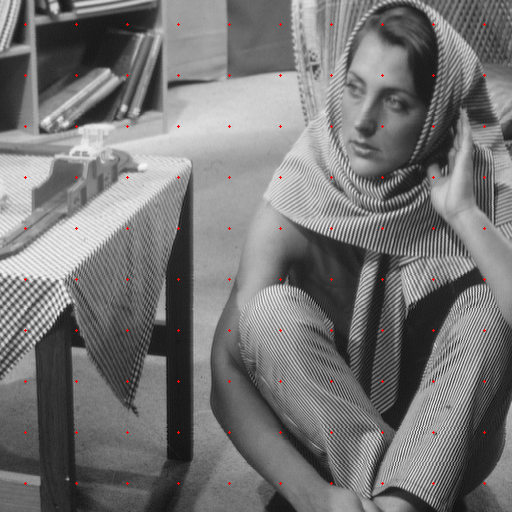
\includegraphics[width=0.6\textwidth]{img/spatiallyUniformSampling.png}
      \caption{Spatially uniform sampling. Red pixels are sampled. Here 100 pixels are sampled, which represents 0.04\% of all pixels}
  \end{figure}
 \item [Incremental sampling (INS)] is an adaptive sampling scheme, meaning that it select points according to the similarity, so that we can have an approximate optimal rank-k subspace of the original image \cite{zhan_improved_2017}.
 \item [Mean-shift segmentation-based sampling] this scheme performs good for complex backgrounds. The method consists in over-segmenting the image into \(n\) regions and only one pixel of each region will be sampled using the spatially closest pixel to the center of the region given a formula in \cite{kao_sampling_2012}.
\end{description}

\subsection{Affinity function}
\label{subsec:kernel-variations}

\paragraph{}
The kernel function \(K_{ij}\) measures the similarity between the pixel \(y_i\) and \(y_j\).
The chosen function is important because it decides on which features the similarity of pixels will be evaluate and the tolerance of it.
To illustrate the impact of the affinity function, here is a list of affinity functions, some with examples of the affinity matrix for certain pixels.
The more a pixel is colored in red, the more similar it is to the selected pixel, with respect to the chosen function.
A blue colored pixel is dissimilar to the considered pixel.

To generate the examples, we use the famous image of Barbara of dimension 512x512 pixels (grayscale image).
We use a spatially uniform sampling technique and select 0.1\% of the pixels.
We show two affinity matrices for some affinity functions, the first one is of a pixel on the table leg and the second on Barbara's eye.
Generating the affinity matrix takes approximately 120 seconds on an Intel i3 processor.

\begin{description}[align=left]
 \item [Spatial Gaussian Kernel] takes only into account the spatial distance between two pixels \cite{siam_slides_2016}.
  The formula of this kernel is
  \[K(x_i, x_j) = exp(-\frac{||x_i - x_j||^2}{h_x^2}).\]

  \begin{figure}[H]
      \centering
      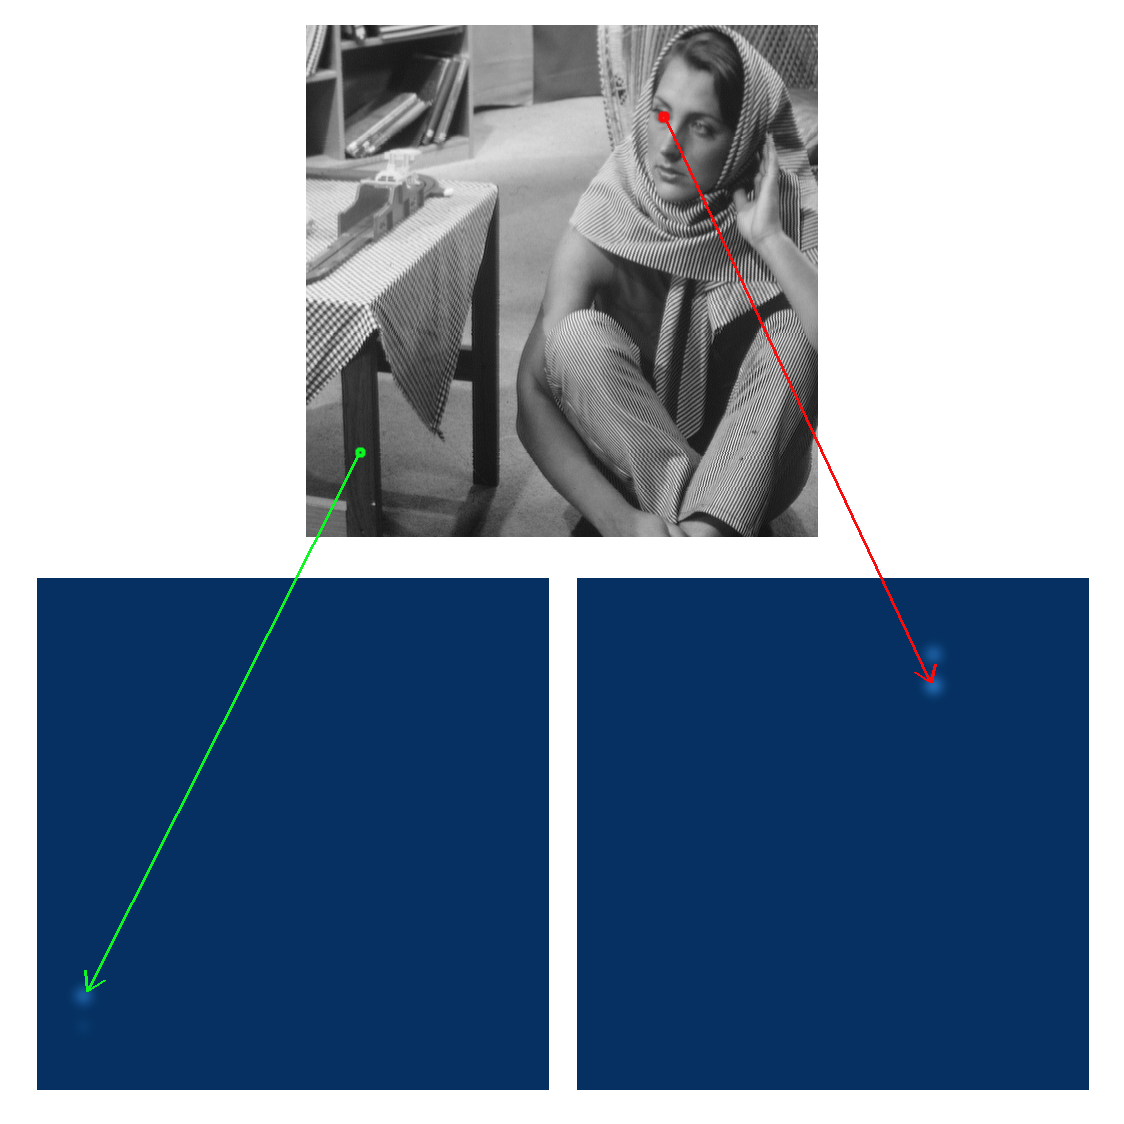
\includegraphics[width=\textwidth]{img/spatialAffinitySigma10.png}
      \caption{Affinity matrices with \(h_x = 10\)}
  \end{figure}

  \begin{figure}[H]
      \centering
      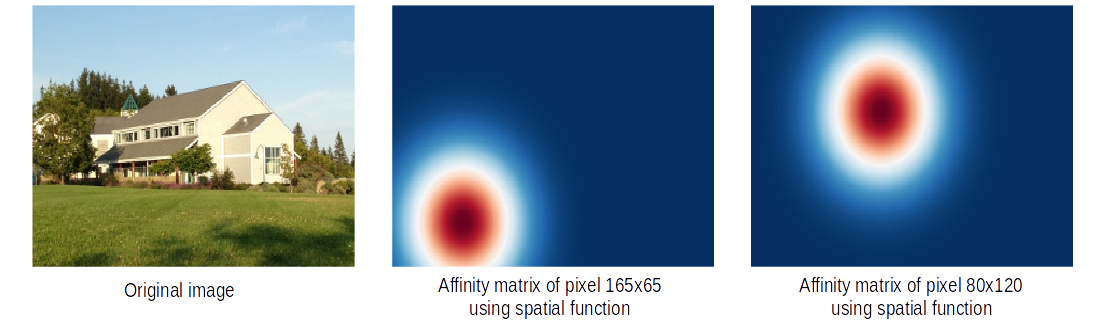
\includegraphics[width=\textwidth]{img/spatialAffinitySigma50.png}
      \caption{Affinity matrices with \(h_x = 50\)}
  \end{figure}

  As we can see, the parameter is influencing on the normalisation of the values and gaussian standard deviation.
  The bigger it is, the more tolerant the spatial distance computation will be.

 \item [Photometric Gaussian Kernel] considers the intensity and color similarity of the pixels \cite{siam_slides_2016}.
  The formula of this kernel is
  \[K(z_i, z_j) = exp(-\frac{||z_i - z_j||^2}{h_z^2}).\]

  \begin{figure}[H]
      \centering
      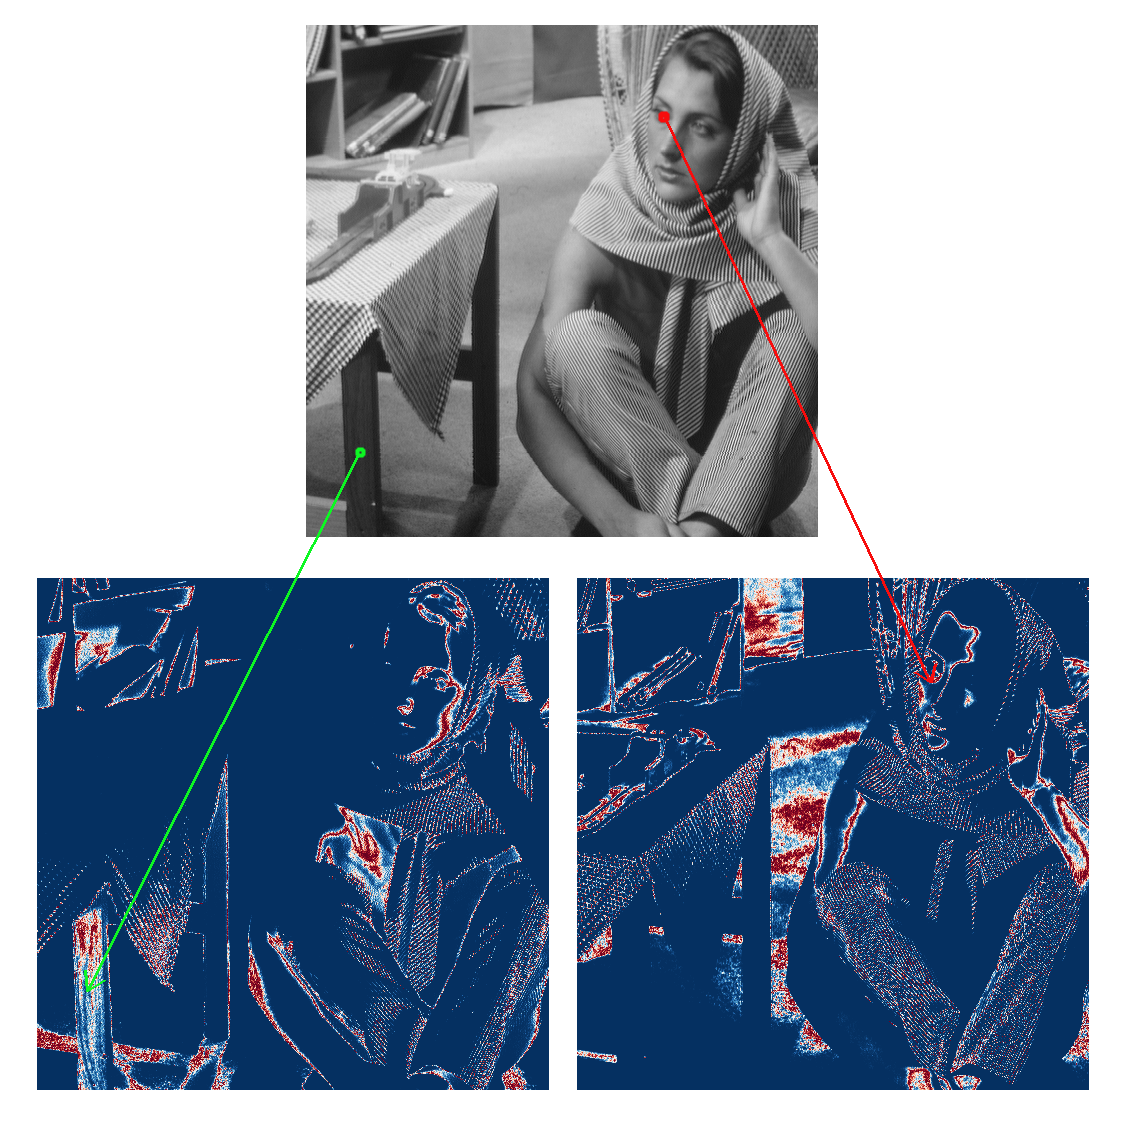
\includegraphics[width=\textwidth]{img/photometricAffinitySigma10.png}
      \caption{Affinity matrices with \(h_z = 10\)}
  \end{figure}

  \begin{figure}[H]
      \centering
      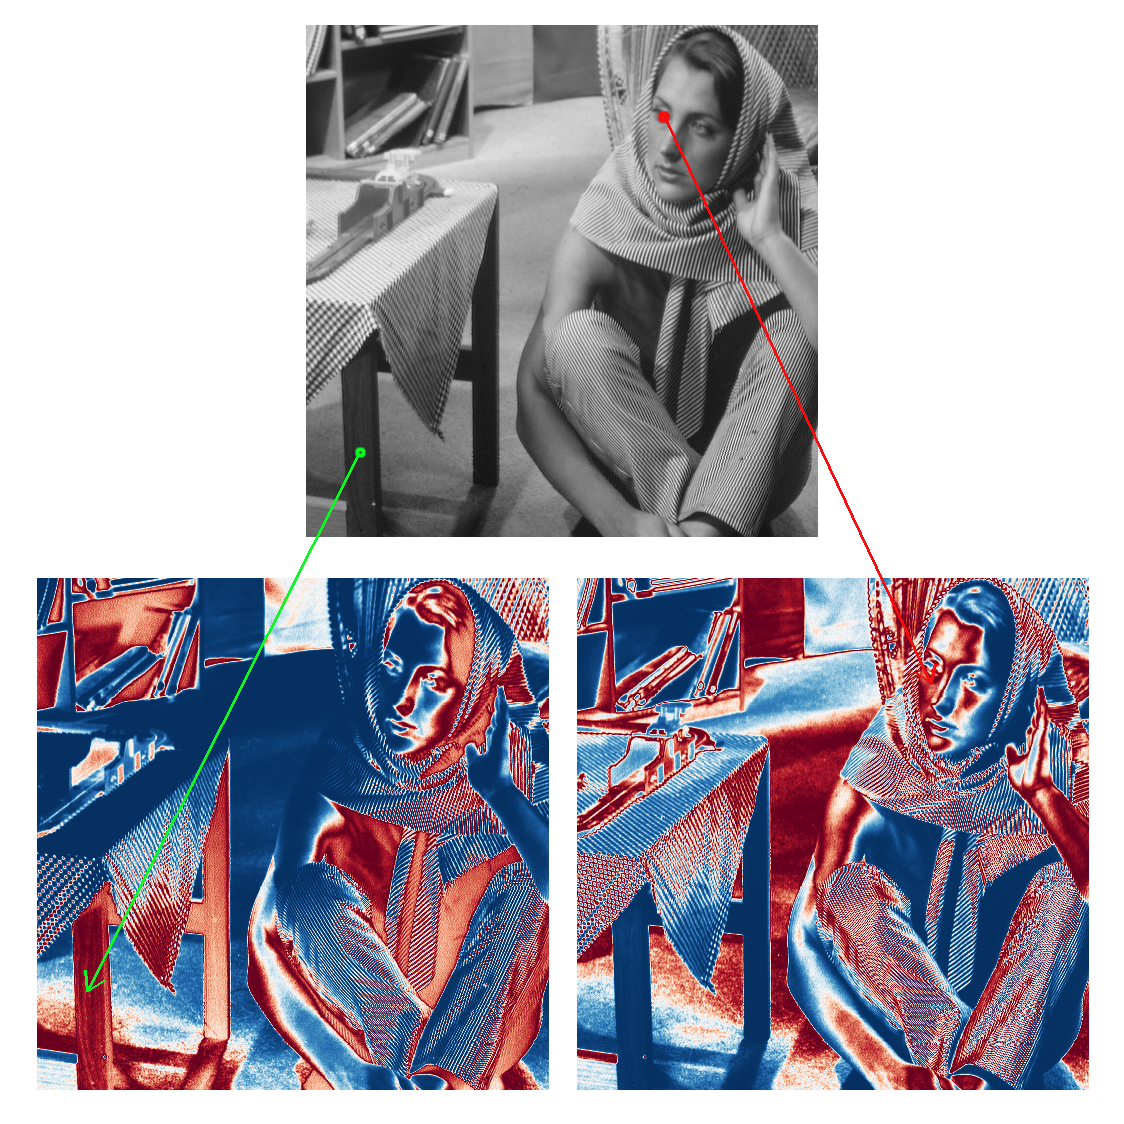
\includegraphics[width=\textwidth]{img/photometricAffinitySigma50.png}
      \caption{Affinity matrices with \(h_z = 50\)}
  \end{figure}

  Generally, the \(h\) parameters in both kernel functions here are smoothing parameters.
  If \(h\) is small, it is more discriminating between the affinity of different pixels.

 \item [Bilateral Kernel] one of the most used kernel which smooths images by a nonlinear combination of the spatial and photometric gaussian kernels \cite{siam_slides_2016} \cite{glide_2014}.

  \begin{figure}[H]
      \centering
      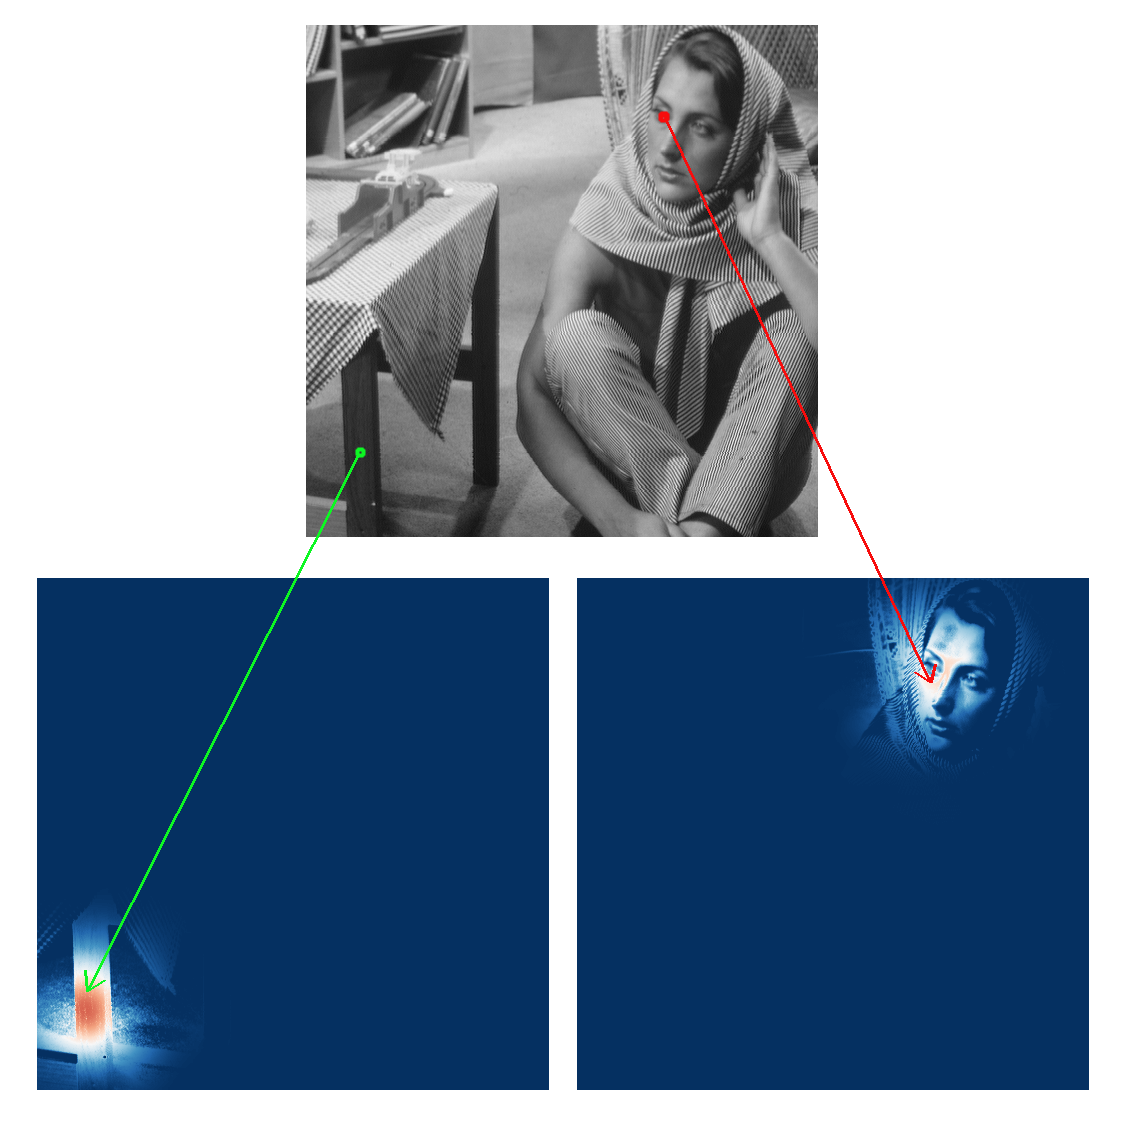
\includegraphics[width=\textwidth]{img/bilateralAffinityPhoto35Spatial50.png}
      \caption{Affinity matrices with \(h_x = 50\) and \(h_z = 35\)}
  \end{figure}

  Remember that each matrix here is only the affinity matrix of one pixel.
  In a very heterogeneous image, the bilateral kernel will be useful to keep the spatial similarity, but with excluding very dissimilar neighbour pixels.

 \item [Non-Local Means (NLM)] is similar to the bilateral kernel, a data-dependent filter, except that the photometric affinity is captured patch-wise \cite{glide_2014}.
 \item [Locally Adaptive Regression Kernel (LARK)] uses the geodesic distance based on estimated gradients \cite{milanfar_symmetrizing_2013} \cite{takeda_kernel_2007}.
\end{description}

\subsection{Graph Laplacians}
\label{subsec:laplacian-variations}

\paragraph{}
The graph Laplacian has multiple possible definitions and each has its own properties.
A good summary can be found in \cite{siam_slides_2016}.
A graph Laplacian can be symmetric which is important for eigendecomposition of the matrix.
It can have a DC eigenvector, which means that the Laplacian has to give 0 if we apply it to a constant image.
And the spectral range, corresponding to the range of the eigenvalues, is important because we can use the filters derived from the Laplacian multiple times, and if the eigenvalues are not between 0 and 1, then the filters tend to be unstable.
With \(K\) being the affinity matrix, \(d_i = \sum_j K_{ij}\) and \(D = diag\{d_i\}\):

\begin{table}[!htbp]
 \centering
 \begin{tabular}{|c|c|c|c|c|}
  \hline
  Laplacian Name & Formula & Symmetric & DC eigenvector & Spectral Range \\
  \hline
  Un-normalised & \(D - K\) & Yes & Yes & [0, n] \\
  \hline
  Normalised & \(I - D^{-1/2}KD^{-1/2}\) & Yes & No & [0, 2] \\
  \hline
  Random Walk & \(I - D^{-1}K\) & No & Yes & [0, 1] \\
  \hline
  ``Sinkhorn" \cite{milanfar_symmetrizing_2013} & \(I - C^{-1/2}KC^{-1/2}\) & Yes & Yes & [0, 1] \\
  \hline
  Re-normalised \cite{milanfar_new_2016} & \(\alpha(D - K)\), \(\alpha = \bigO(n^{-1})\) & Yes & Yes & [0, 1] \\
  \hline
 \end{tabular}
\end{table}

Generally, it is a good practice to stick to one definition of the Laplacian.

\section{Discussions and remarks}

\paragraph{}
For our implementations, we choose to focus first on grayscale images.
We sample the picture using the spatially uniform techniques which yields good results for natural images since they contain redundancy.
The affinity function the photometric gaussian kernel with the parameter \(h = 10\).

We want to use the re-normalised Laplacian definition to build a smoothing/denoising data-dependent filter.
The filter is built such as
\[\Lapl = I-W.\]
Our Laplacian operator formulation is \(\Lapl = \alpha (D-K)\), so \(I-W = \alpha (D-K)\) and finally
\[W = I + \alpha (K-D).\]
This is supported by \cite{milanfar_new_2016}.
However, as final step, we want to approximate \(W\) by \(\hat{W}\) through its orthonormal eigenvectors and eigenvalues.
For this step, \(W\) has to be both symmetric and positive definite.
The latter condition is not satisfied with this Laplacian definition.
Indeed, \(W\) can contain negative values and the eigenvalues are both positive and negative.
So \(W\) is an indefinite matrix.
We will stick with for now stick with the ``Sinkhorn" \cite{milanfar_symmetrizing_2013} definition of the graph Laplacian.

\paragraph{Pixel degree}

An interesting matrix that can be observed is the degree of the pixels.
A pixel, in our case, is a node of the graph, so we sum the weights of outgoing edges from each node.
On the picture below, red pixels indicate that the pixel has a lot of similarity with all other pixels in the image, which can be roughly interpreted as the pixel is a common one:

\begin{figure}[H]
    \centering
    \begin{subfigure}[b]{0.45\textwidth}
        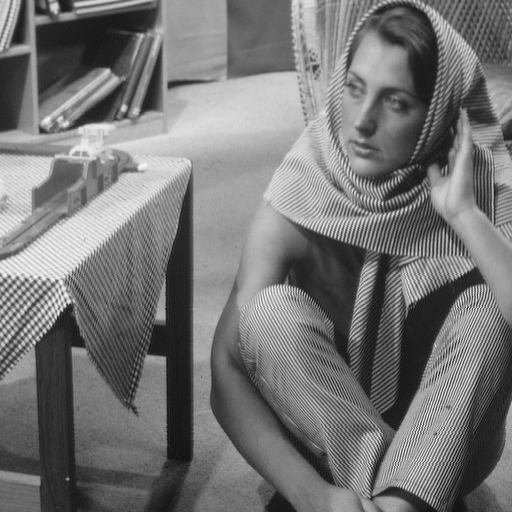
\includegraphics[width=\textwidth]{img/barbara.png}
        \caption{Original image}
    \end{subfigure}
    \begin{subfigure}[b]{0.45\textwidth}
        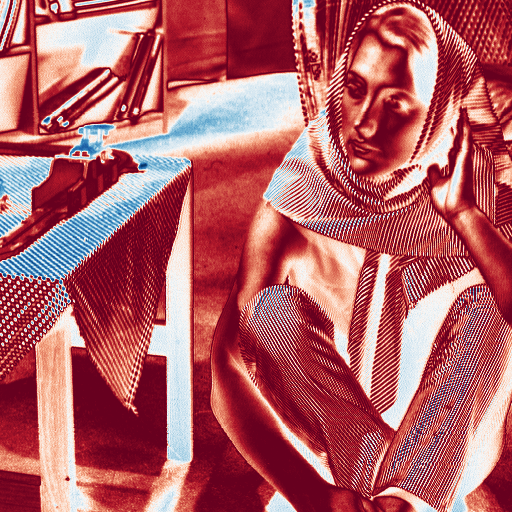
\includegraphics[width=\textwidth]{img/pixelDegrees.png}
        \caption{Pixel degrees}
    \end{subfigure}
\end{figure}

We observe that the most uncommon pixels are very light ones and very dark ones in this image.
